\documentclass{article}

\usepackage{amssymb}
\usepackage{verbatim}
\usepackage[francais,english]{babel}
\usepackage{graphicx}
\usepackage{graphics}
\usepackage{lineno}
\usepackage[latin1]{inputenc}
\usepackage[table]{xcolor}
\usepackage[]{natbib}
\usepackage[]{multirow}
\usepackage[]{a4wide}
\usepackage{fancyhdr}
\usepackage{lastpage}
\usepackage{amsmath}
\usepackage{lineno}
%\linenumbers

%\definecolor{light-gray}{gray}{0.8}
%\linenumbers
%\frontmatter
%\pagestyle{arabic}

\begin{document}
%\pagenumbering{arabic}
%\cfoot{\thepage/\pageref{LastPage}}
%\setcounter{page}{1}

\baselineskip 0.8cm

\title{{\tt TESS3}: Fast Inference of Spatial Population Structure and Genome Scans for Selection} 

\date{}

\author{Kevin Caye$^1$ \and Timo M. Deist$^1$ \and Helena Martins$^1$ \and Olivier Michel$^2$ \and Olivier Fran\c cois$^1$}

\maketitle

\begin{center}
$^1$Universit\'e Grenoble-Alpes, Centre National de la Recherche Scientifique, TIMC-IMAG UMR 5525, Grenoble, 38042, France.\\
$^2$Universit\'e Grenoble-Alpes, Centre National de la Recherche Scientifique, GIPSA-lab UMR 5216, Grenoble, 38042, France.\\
\end{center}

\noindent{Running Title: {\tt TESS3}: Inference of Spatial Population Structure\\}

\noindent{\bf Keywords:} Inference of Population Structure, Geographic Variation, 
Genome Scans for Selection, Control of False Discoveries.

\vspace{1cm}

{\noindent Corresponding Author: Olivier Fran\c cois \\
Universit� Grenoble-Alpes,\\ 
TIMC-IMAG,  UMR CNRS 5525,\\
Grenoble, 38042, France.\\
+334 56 52 00 25 (ph.)  \\
+334 56 52 00 55 (fax)  \\
 \texttt{olivier.francois@imag.fr}}


\clearpage
\newpage 
%
%
%
%
\begin{center}{\bf
Abstract}
\end{center}

Geography and landscape are important determinants of genetic variation in natural populations, and severalancestry estimation methods have been proposed to investigate population structure using genetic and geographic data simultaneously. Those approaches are often based on computer-intensive stochastic simulations, and do not scale with the dimensions of the data sets generated by high-throughput sequencing technologies. There is a growing demand for faster algorithms able to analyze genome-wide patterns of population genetic variation in their geographic context.
                                    

In this study, we present TESS3, a major update of the spatial ancestry estimation program TESS. By combining machine learning and spatial statistical methods, we provide estimates of ancestry coefficients with accuracy comparable to TESS and with run-times much faster than TESS. In addition, the TESS3 program can be used to perform genome scans for selection, and separate adaptive from non-adaptive genetic variation using ancestral allele frequency differentiation tests. The main features of TESS3 are illustrated using simulated data and analyzing genomic data from European lines of the plant {\it Arabidopsis thaliana}.

\clearpage
\newpage 



     
  \section{Introduction}


Since the early developments of population genetics, geography has been recognized as one of the major determinants of genetic variation in natural populations~\citep{wright1943isolation,malecot1948mathematics,kimura1964stepping,cavalli1994history,
epperson2003geographical}. For these populations, spatial patterns of genetic variation can be influenced by landscape barriers, geographical distances and by the processes of divergence and admixture resulting from the colonization of new areas. In addition, analyzing spatial patterns of genetic variation has been a long-standing goal of evolutionary biogeography, molecular ecology, landscape genetics, and conservation biology~\citep{segelbacher2010applications,manel2010perspectives}.


Statistical approaches to analyze spatial patterns of genetic variation often rely on the inference of population genetic structure from multi-locus genotype data, which is commonly performed using the Bayesian approach implemented in the computer program {\tt STRUCTURE}~\citep{pritchard2000inference}.  Assuming $K$ unobserved ancestral gene pools, {\tt STRUCTURE} computes allele frequencies in each pool, and estimates individual {\it ancestry coefficients} representing the proportion of an individual genome that originates from each pool. Using {\tt STRUCTURE}, ancestry coefficients are estimated without prior knowledge on geographic proximity among individuals. 

The approach implemented in {\tt STRUCTURE} has been substantially improved by a number of approaches that include spatial proximity information based on individual geographic coordinates (reviewed by~\cite{franccois2010spatially}). Among those spatially explicit approaches, the computer program {\tt TESS} is one of the most frequently used algorithms~\citep{chen2007bayesian,franccois2006bayesian}. In the {\tt TESS} model, ancestry proportions are continuously distributed over geographic space, and the parameters that specify the shape of the clines are estimated from the genetic and the geographic data. Using geographic information, {\tt TESS} provides better estimates of ancestry coefficients than {\tt STRUCTURE} when the levels of ancestral population divergence are low (Durand et al. 2009).  

The Bayesian approaches implemented in {\tt STRUCTURE} and {\tt TESS} rely on Markov Chain Monte Carlo algorithms. Monte Carlo algorithms are based on computer intensive stochastic simulations, and have the advantage of sampling the posterior distribution of the model parameters. However the application of stochastic algorithms can be difficult when the data include more than a few hundreds of individuals or a few thousands of allelic markers. With the availability of next generation sequencing data, there is a need to analyze genotypic matrices that represent thousands of individuals and hundreds of thousands of markers. While fast versions of {\tt STRUCTURE} have already been proposed~\citep{raj2014faststructure, frichot2014fast, alexander2011linking, wollstein2015detecting}, developing fast and accurate estimation algorithms for ancestry coefficients in a geographic framework remains an important computational challenge.

In this study, we present a spatially explicit algorithm that provides fast estimation of ancestry coefficients with accuracy comparable to {\tt TESS} 2.3~\citep{durand2009spatial}. The new algorithms are based on least-squares optimization and on geographically constrained non-negative matrix factorization~\citep{cai2011graph,frichot2014fast}. These improvements of {\tt TESS} are implemented in the computer program {\tt TESS3}. We show that {\tt TESS3} is substantially faster than {\tt TESS} 2.3, with an increase in computational speed of one or two orders of magnitude. In addition, we show that ancestral allele frequencies are correctly estimated, and we illustrate the use of the {\tt TESS3} program to perform genome scans for selection based on ancestral allele frequency differentiation. To illustrate our approach, {\tt TESS3} was applied to genomic data from European lines of the model species {\it Arabidopsis thaliana} for which an individual-based sampling design was available~\citep{atwell2010genome}.


%Cavalli-Sforza, L. L., Menozzi, P., Piazza, A. (1994). The history and geography of human genes. Princeton university press.



%Epperson, B. K. (2003). Geographical Genetics. Princeton University Press.



%Kimura, M.,  Weiss, G. H. (1964). The stepping stone model of population structure and the decrease of genetic correlation with distance. Genetics, 49(4), 561.



%Wright, S. (1943). Isolation by distance. Genetics, 28(2), 114.



%Segelbacher, G., Cushman, S. A., Epperson, B. K., Fortin, M. J., Francois, O., et al. (2010). Applications of landscape genetics in conservation biology: concepts and challenges. Conservation Genetics, 11(2), 375-385.



%Raj A, Stephens M, Pritchard JK: fastSTRUCTURE: Variational Inference of Population Structure in Large SNP Data Sets. Genetics 2014, 197:573-589.






\section{Materials and Methods}
\label{sec:MM}
% introduction

The computer program {\tt TESS3} computes ancestry estimates for large genotypic matrices using the geographic coordinates of sampled individuals. The program also returns locus-specific estimates of ancestral genotypic frequencies, and computes locus-specific estimates of a population-based differentiation statistic that can be used in genome scans for adaptive alleles. The {\tt TESS3} program is particularly suited to the analysis of large genomic data sets, for which the number of loci ($L$) ranges between thousands to hundreds of thousands genetic polymorphisms and the number of individuals ($n$) ranges between hundreds to thousands individuals.


\paragraph{Input data.} 
{\tt TESS3} requires  that the data consists of $n$ multi-locus genotypes and two geographic coordinates for each genotype. A genotypic matrix, $X$, records allelic data for each individual ($i$) and each locus ($\ell$).  With data representing single nucleotide polymorphisms (SNPs), the genotypic matrix records the number of derived or mutant alleles at each locus. Considering autosomes in a diploid organism, the genotype at locus $\ell$ corresponds to the number of derived alleles at this locus, which is encoded as an integer number 0, 1 or 2. Standard format {\tt geno} is accepted by the program, and it can also process other types of allelic data, such as short tandem repeats or amplified fragment length polymorphisms.  Geographic coordinates can be expressed using several coordinate systems, for example longitude and latitude, and they are provided in a separate file.


\paragraph{Geographically constrained least-squares estimates of ancestry coefficients.} 

As in the {\tt TESS} 2.3 or in the {\tt STRUCTURE} model, {\tt TESS3} supposes that the genetic data originate from the admixture of $K$ ancestral populations, where $K$ is unknown. Following standard notations, we let $Q_{ik}$ denote the fraction of individual $i$'s genome that originates from the ancestral population $k$, and $G_{k\ell}(j)$ represents the frequency of genotype $j$ at locus $\ell$ in population $k$. The $Q$-matrix, $Q = (Q_{ik}) $, is the matrix of individual ancestry coefficients ($n\times K$ dimensions). The $G$-matrix, $G= (G_{k\ell}(j))$, is the matrix of ancestral genotype frequencies. The dimension of $G$ is equal to $K\times (p+1) L$ where $p$ is the ploidy of the studied organism genome. 

To compute estimates for the $Q$ and $G$ matrices, {\tt TESS3} builds a nearest-neighbor graph based on the sampling sites and runs a least-squares minimization algorithm. More specifically, the estimates are obtained by using a graph-regularized matrix factorization approach~\citep{cai2011graph}. In this approach, the estimates of $Q$ and $G$ are obtained after solving the following constrained least-squares problem

$$
(\hat Q, \hat G) = \arg \min {\rm LS}(Q, G) \, ,
$$

\noindent where

\begin{equation}\label{eq:LS}
{\rm LS}(Q, G) =  \|  \tilde{X} - QG \|^2_{\rm F}   +   \alpha   \sum_{s_i \sim s_j}   w_{ij} \|  Q_{i.}  - Q_{j.} \|^2   \, , 
\end{equation}

\noindent and $Q$ and $G$ are non-negative matrices such that, for all $i$ and $\ell$, we have  

$$
\sum_{k=1}^K Q_{ik} = 1  \qquad \sum_{j=0}^{p} G_{i\ell}(j) = 1 \, .
$$

\noindent In this equation, $\| M \|_{\rm F}$ denotes the Frobenius norm of a matrix $M$,  $\| V \|$ is the Euclidean norm of a vector $V$, $\alpha$ is a non-negative {\it regularization parameter}, and $\tilde{X}_{i\ell}$ records the absence/presence of each particular genotype at locus $\ell$ for individual $i$~\citep{frichot2014fast}. In our algorithm, we used $3$ bits of information to encode each 0, 1 or 2 value as an indicator of a heterozygote or a homozygote locus. Thus, the dimension of the $\tilde{X}$-matrix is $n \times (p+1) L$. The summation on the right-hand side of the second term runs over all pairs of sites, $s_i \sim s_j$ , sharing an edge in the nearest-neighbor graph. The number of neighbors in the graph was set to represent $5\%$ of total connections.
The quantity $w_{ij}$ is a weight that decreases with geographic distance between sampling sites as follows

\begin{equation} 
w_{ij} =\exp( -  d(s_i, s_j)^2 / \bar{d^2}  ) \, ,  
\end{equation}

\noindent where $d$ is the Euclidean distance, and $\bar{d}$ is the average distance computed over the neighboring sites in the sample. More specifically, the weight of an edge in the nearest-neighbor graph is related to the Laplace-Beltrami operator on a manifold~\citep{belkin2003laplacian}. 
The parameter $\alpha$ controls the regularity of ancestry estimates over the geographic space. Large values of $\alpha$ imply that ancestry coefficients have similar values for nearby individuals. In the algorithm, the regularization parameter $\alpha$ is equal to $c \times nL(p+1) / \sum w_{ij}$ . The default value of $c$ is $0.1\%$.



Mathematically, {\tt TESS3} runs a {\it geographically constrained} non-negative matrix factorization algorithm for the data matrix $\tilde{X}$. Least squares minimization is performed using the Alternating Non-negativity-constrained Least Squares (ANLS) algorithm with the active set (AS) method following the approach used in the computer program {\tt sNMF}~\citep{frichot2014fast,kim2011fast}. The ANLS-AS algorithm starts with the initialization of the $Q$ matrix, and then computes a non-negative matrix $G$ that minimizes the quantity 
$${\rm LS}_1(G) = \|X - QG \|_F^2 \, .$$
The obtained solution is normalized so that its entries satisfy the probabilistic constraints for genotypic frequencies. Given $G$, the $Q$-matrix is computed after minimizing the following quantity 
 
$${\rm LS}_2(Q) = 
\left|\left|
\left(
    \begin{array}{c}
      {\rm Vec}(\tilde{X}^T) \\
      0
    \end{array}
  \right)
   -  
   \left(
   \begin{array}{c}
      {\rm Id} \otimes G^T \\
      \sqrt{\alpha} ~ \Gamma \otimes {\rm Id}
    \end{array}
  \right) {\rm Vec}(Q^T)  
   \right|\right|_F^2
   \, ,
$$

\noindent where ${\rm Vec}(\tilde{X})$ denotes the vectorization of the matrix $\tilde{X}$ formed by stacking the columns of $\tilde{X}$ into a single column vector, $\Gamma$ is the Cholesky decomposition of the graph Laplacian associated with the weights of the graph~\citep{chung1997spectral}. Iterations are stopped when the relative difference between two successive values of ${\rm LS}(Q,G)$  is lower than a tolerance threshold of $\epsilon$. The default value for $\epsilon$ equals $10^{-7}$.
  


The number of ancestral populations, $K$, is chosen after the evaluation of the cross-entropy criterion for each $K$~\citep{frichot2014fast}. The choice of $K$ is then based on a cross-validation method that  partitions the genotypic matrix entries into a training set and a test set in which 5$\%$ of all entries are masked to the algorithm. The objective of the cross-entropy criterion is to compare genotypic frequencies predicted from the training set to those computed from the test set at each locus. Smaller values of the criterion indicate better estimates for {\tt TESS3}.

\paragraph{Outlier tests.} 

In addition to the inference of spatial population structure, {\tt TESS3} can perform genome scans for selection when the program is applied to large genomic data sets. More specifically, {\tt TESS3} uses the ancestral genotype frequency matrix, $G$, to derive the allele frequencies in the $K$ ancestral populations. Then the algorithm evaluates a locus-specific $F_{\rm ST}$-statistic based on the estimated ancestral allele frequencies.
Using standard population genetic theory, $F_{\rm ST}$-statistics can be transformed into squared $t$-scores, and $p$-values can be computed using a chi-square distribution with one degree of freedom~\citep{weir1990genetic}. To correct test inflation due to neutral population structure, the $t$-scores are recalibrated using estimates of the inflation factor that are graphically determined
on the basis of quantile-quantile plots of $p$-values~\citep{devlin1999genomic}.
Multiple testing issues can be addressed by applying the Benjamini-Hochberg algorithm to the recalibrated $p$-values with expected levels of false discovery rate~\citep{benjamini1995controlling}.  

\paragraph{Simulated data sets and program runs.} 

%We created simulated data sets containing 200 admixed genotypes with levels of ancestry that varied continuously accross geographic space. To generate the data,  we first used the computer program {\tt MS} to perform coalescent simulations of neutral and outlier SNPs under models of structured populations (2-island models, Hudson 2002). The justification for using neutral migration-drift equilibrium models for simulating selection is that loci with selection coefficient $s$, have an effectively reduced migration rate, $m_{\rm s}$ as compared to the neutral migration $ m$ in migration-selection-drift equilibrium models (Bazin et al. 2010). 

%Considering two source populations under a migration-drift equilibrium model, we set the neutral migration rate to the value $4m N = 20$. The number of loci was varied in the range $L = 2 - 100$k, and the proportion of outlier loci was equal to $5\%$. Outlier loci were generated using values of the effective migration rate in the range $4m_{\rm s} N = 2-10$. One hundred genotypes were sampled from each source population, and admixed genotypes were created according to a longitutinal gradient of ancestry (Durand et al. 2009, Fran�ois and Durand 2010). Individuals at the each extreme of the longitunal range were representative of ancestral populations, while individuals at the center of the range shared intermediate levels of ancestry in the two source populations. 


We created simulated data sets containing 200 admixed genotypes with levels of ancestry that varied continuously across geographic space. To generate the data,  we used the computer program {\tt MS} to perform coalescent simulations of neutral and outlier SNPs under island models with two populations~\citep{hudson2002generating}. One hundred genotypes were sampled from each source population, and admixed genotypes were created according to a longitudinal gradient of ancestry~\citep{durand2009spatial,franccois2010spatially}. Individuals at each extreme of the longitunal range were representative of ancestral populations, while individuals at the center of the range shared intermediate levels of ancestry in the two source populations. The number of loci was varied in the range $L = 1$k-$50$k SNPs.

Our first series of simulations considered selectively neutral SNPs and used migration parameters, $M = 4mN_{e}$, between $M = 0.01$ and $M = 10$. The population differentiation statistic, $F_{\rm ST}$, ranged from $0.0076$ to $0.42$. Our second series of simulations included a proportion of outlier SNPs equal to $5\%$. Outlier loci were generated using two values of the effective migration rate $4m_{\rm s} N = 0.1$ and $4m_{\rm s} N = 1$. In simulations with outlier loci, the neutral migration rate was set to the value $4m N = 20$. The justification for using neutral migration-drift equilibrium models for simulating selection is that loci with selection have an effectively reduced migration rate, as compared to the neutral migration $m$ in migration-selection-drift equilibrium models~\citep{bazin2010likelihood}. 
 
 The simulated data were analyzed to compare {\tt TESS3} estimates to those of {\tt TESS} 2.3~\citep{durand2009spatial}. The number of ancestral populations ranged from $K=1$ to $K=6$.  Each run was replicated five times for each computer program.  The number of cycles in the Markov chain Monte Carlo algorithm of {\tt TESS} 2.3 was set to 1,000, and the number of ancestral population was determined using the deviance information criterion. All other parameters were set to their default values. Statistical errors were measured as root mean squared errors (RMSE) between the estimated $Q$-matrix and the matrix of coefficients ($Q^0$) that were used to generate the data
   
$$
{\rm RMSE} =  \left(    \frac{1}{nK} \sum_{i =1}^n \sum_{k=1}^K   (Q_{ik} - Q_{ik}^{0})^2   \right)^{1/2} \, .
$$ 
   
\noindent A similar RMSE criterion was defined for comparing the estimates of $G$ matrices obtained from {\tt TESS3} or {\tt TESS} 2.3 to the estimates of the ancestral genotypic frequency matrix resulting from the coalescent simulations.


\paragraph{{\it Arabidopsis thaliana} data.} 


We applied {\tt TESS3} to genomic data from 170 European lines of the model plant {\it Arabidopsis thaliana} genotyped for 216k SNPs~\citep{atwell2010genome}. For these data, we determined the number of ancestral populations using the cross-entropy criterion, and we computed ancestry estimates for the sample. We also used {\tt TESS3} to perform  a genome scan for selection on chromosome 5 using $K = 3$ ancestral populations (54k SNPs).



  

\section{Results}

\paragraph{Comparison of ancestry estimates.}
We used computer simulations of admixed populations to evaluate the ability of {\tt TESS3} to reproduce the ancestry estimates of {\tt TESS} 2.3 using known individual ancestry proportions from two ancestral gene pools. Simulating 2k unlinked SNPs, we varied the level of ancestral population differentiation, measured by $F_{\rm ST}$, to create difficult as well as easier data sets.  For all data sets, the information criterion of each version of {\tt TESS} led to $K = 2$ clusters. Statistical errors, measured by RMSEs for estimated $Q$ and $G$ matrices, ranged between $0.02$ and $0.15$ (Figure 1). Statistical errors increased as the levels of differentiation between the two source populations decreased, but remained in an acceptable range for values of $F_{\rm ST}$ lower than $0.016$. Overall, the statistical performances were of the same order for both versions of {\tt TESS}. 

\paragraph{Run-time analysis.}
Next we compared the run-times of {\tt TESS3} and {\tt TESS 2.3} for increasing values of the number of ancestral populations and increasing numbers of loci. For {\tt TESS 2.3} the total number of cycles in the MCMC algorithm was set to 1,000, a value for which the Monte-Carlo sampler reached its equilibrium state. Run-times were averaged over distinct random seed values for each $K$ and number of loci. For both algorithms, the run-times increased with the number of loci and with the number of ancestral populations (Figure 2). For $L = 10$k loci, {\tt TESS3} and {\tt TESS 2.3} runs took less than 6 minutes on an Intel Xeon 2.40 GHz CPU. With $L = 50$k loci and $K = 5$ ancestral populations, {\tt TESS 2.3} took on average 30 minutes to complete a single run, whereas the {\tt TESS3} average run-time was about 4 minutes.
  

\paragraph{Outlier detection with {\tt TESS3}.}

We evaluated the capacity of {\tt TESS3} to detect outlier loci on simulated data containing $5\%$ of outlier loci. For each locus, we performed a population differentiation test based on the estimated ancestral allele frequencies. For a data set with $m_{\rm s}/m = 0.005$, the estimate of the genomic inflation factor was equal to $\lambda = 4.4$. For a data set with $m_{\rm s}/m = 0.05$ this value was equal to $\lambda = 10.0$. For these values of $\lambda$, the observed levels of the false discovery rate were close to their expected values. The power to reject the null hypothesis was lower when the intensity of selection was low (Table 1). For an expected FDR of $q=0.1$, the power of the test was approximately equal to $60\%$ for the higher selection rate and it was equal to $20\%$ for the lower selection rate. 




\paragraph{Biological data analysis.}
We applied {\tt TESS3} to a genomic data set of 170 European lines of {\it Arabidopsis thaliana} (216k SNPs). The cross-entropy curve exhibited a change in curvature for $K = 3$-4 clusters. For $K = 3$, the western cluster grouped all lines from the British Isles, France and Iberia. The eastern cluster grouped all lines from Central, Eastern Europe and Southern Sweden. Fourteen northern Scandinavian accessions were grouped into a separate population (Figure 3A). Those results were consistent with those obtained with {\tt TESS 2.3}. The average run-time of {\tt TESS3} was about 5 minutes whereas each {\tt TESS 2.3} run took about 2 hours. Then we performed a genome scan for selection based on population differentiation in the three ancestral populations detected by {\tt TESS3}. The genomic inflation factor was equal to $\lambda = 30.0$. The histogram of corrected $p$-values provided evidence that confounding errors were correctly removed (Figure 4A).  The Manhattan plot exhibited islands of strong differentiation around positions 8,510 kb, 6,944 kb, 6,969 kb and 26,155 kb in the chromosome 5 (Figure 3B). The top hits in the candidate list corresponded to genic SNPs. In particular, we discovered genes involved in defense response ({\it VSP1}), photoperiodism, flowering and root development ({\it WAV2})~\citep{mochizuki2005arabidopsis}. The derived allele in the {\it VSP1} gene was at high frequency in Eastern Europe and almost absent from Western Europe and Northern Scandinavia. The derived allele in the {\it WAV2} gene was at high frequency in the Iberian peninsula and at low frequency in Eastern Europe and Northern Scandinavia (Figure 4B). 



%\clearpage
\newpage


\section{Results}
\paragraph{Statistical errors} We used coalescent simulations of neutral
polymorphisms under spatial models of admixture to compare the statistical
errors of the AQP and APLS estimates with those of the {\tt tess3}
algorithm~\citep{Caye2016}. The ground truth for the $Q$-matrix (${\bf Q}_0$)
was computed from the mathematical model for admixture proportions used to
generate the data. For the $G$-matrix, the ground truth matrix (${\bf G}_0$) was
computed from the empirical genotype frequencies in the two population samples
before an admixture event. The root mean squared errors (RMSE) for the ${\bf Q}$
and ${\bf G}$ estimates decreased as the sample size and the number of loci
increased (Figure~\ref{fig:fig1}). For all algorithms, the statistical errors were generally
small when the number of loci was greater than $10$k SNPs. Those results
provided evidence that the three algorithms produced equivalent estimates of the
matrices ${\bf Q}_0$ and ${\bf G}_0$. The results also provided a check
that the APLS and {\tt tess3} algorithms converged to the same estimates as
those obtained after the application of the AQP algorithm, which is guaranteed
to converge mathematically.


\paragraph{The benefit of including spatial information in algorithms} Using
neutral coalescent simulations of spatial admixture, we compared the statistical
estimates obtained from a spatial algorithm (APLS) and a non-spatial algorithm
(sNMF, Frichot et al. 2014). For various levels of ancestral population
differentiation, estimates obtained from the spatial algorithm were more
accurate than for those obtained using non-spatial approaches (Figure~\ref{fig:fig2}). For
the larger samples, much finer population structure was detected with the
spatial method than with the non-spatial algorithm (Figure~\ref{fig:fig2}).

In simulations of outlier loci, we used the area under the precision-recall
curve (AUC) for quantifying the performances of tests based on the estimates of
ancestry matrices, {\bf Q} and {\bf G}. In addition, we computed AUCs for
$F_{\rm ST}$-based neutrality tests using truly ancestral genotypes. As they
represented the maximum reachable values, AUCs based on truly ancestral
genotypes were always higher than those obtained for tests based on
reconstructed matrices. For all values of the relative selection intensity, AUCs
were higher for spatial methods than for non-spatial methods (Figure~\ref{fig:fig3}, the
relative selection intensity is the ratio of migration rates at neutral and
adaptive loci). For high selection intensities, the performances of tests based
on estimates of ancestry matrices were close to the optimal values reached by
tests based on true ancestral frequencies. These results provided evidence that
including spatial information in ancestry estimation algorithms improves the
detection of signatures of hard selective sweeps having occurred in unknown
ancestral populations.

\paragraph{Sensitivity of estimates to spatial measurements.} Next, we used the
simulated data sets to evaluate the robustness of APLS estimates to inaccurate
measurements of spatial coordinates. To this aim, Gaussian noise was added to
truly observed geographic coordinates by considering values of the
noise-to-signal ratio ranging from 0 to 3. We computed variograms in all
cases, and found that the spatial signal was removed from simulations with a
noise-to-signal ratio of ??? ($\sigma \approx 0$), while the signal was still
observable with a noise-to-signal ratio of 1.
%% TODO paragraph quand fig OK
A noise-to-signal ratio of 1 increased statistical errors in the $Q$-matrix
estimates, but the RMSEs remained generally lower than for methods without
spatial coordinates ($\alpha = 0$ and sNMF, Figure~\ref{fig:fig2_5}). For a noise-to-signal ratio
of 3, errors were higher than for methods without spatial coordinates
(Figure~\ref{fig:fig2_5}). To a large extent, estimates from the APLS algorithm
were robust to uncertainty in spatial measurements. Standard graphical tests
such as a variogram analysis can help deciding whether our spatially explicit
algorithm is useful or not.


\paragraph{Runtime and convergence analyses} We subsampled a large SNP data set
for {\it A. thaliana} ecotypes to compare the convergence properties and
runtimes of the {\tt tess3}, AQP, and APLS algorithms. In those experiments, we
used $K = 6$ ancestral populations, and replicated 5 runs for each simulation.
For $n = 100-600$ individuals ($L = 50$k SNPs), the APLS algorithm required more
iterations (25 iterations) than the AQP algorithm (20 iterations) to converge to
its solution (Figure~\ref{fig:fig4}). This was less than for {\tt tess3} (30 iterations). For
$L = 10-200$k SNPs ($n = 150$ individuals), similar results were observed. For
$50$k SNPs, the runtimes were significantly lower for the APLS algorithm than
for the {\tt tess3} and AQP algorithms. For $L = 50$k SNPs and $n = 600$
individuals, it took on average 1.0 min for the APLS and 100 min for the AQP
algorithm to compute ancestry estimates. For {\tt tess3}, the runtime was on
average 66 min. For $L = 100$k SNPs and $n = 150$ individuals, it took on
average 0.6 min (9.0 min) for the APLS (AQP) algorithm to compute ancestry
estimates. For {\tt tess3}, the runtime was on average 1.3 min. For those
values of $n$ and $L$, the APLS algorithm implementation ran about 2 to 100
times faster than the other algorithm implementations.
 
\paragraph{Human data analysis} To evaluate a case of model misspecification
%% TODO
 
\paragraph{Application to European ecotypes of {\it Arabidopsis thaliana}} We
used the APLS algorithm to survey spatial population genetic structure and
perform a genome scan for adaptive alleles in European ecotypes of the plant
species {\it A. thaliana}. The cross validation criterion decreased rapidly from
$K=1$ to $K=3$ clusters, indicating that there were three main ancestral groups
in Europe, corresponding to geographic regions in Western Europe, Eastern and
Central Europe and Northern Scandinavia. For $K$ greater than four, the values
of the cross validation criterion decreased in a slower way, indicating that
subtle substructure resulting from complex historical isolation-by-distance
processes could also be detected (Figure~\ref{fig:fig5}). The spatial analysis provided an
approximate range of $\sigma = 150$km for the spatial variogram (Figure~\ref{fig:fig5}).
Figure~\ref{fig:map} displays the $Q$-matrix estimate interpolated on a geographic map of
Europe for $K = 6$ ancestral groups. The estimated admixture coefficients
provided clear evidence for the clustering of the ecotypes in spatially
homogeneous genetic groups.

\paragraph{Targets of selection in {\it A. thaliana} genomes} Tests based on the
$F^Q_{\rm ST}$ statistic were applied to the 241k SNP data set to reveal new
targets of natural selection in the {\it A. thaliana} genome. {\it A. thaliana}
occurs in a broad variety of habitats, and local adaptation to the environment
is acknowledged to be important in shaping its genetic diversity through
space~\citep{Hancock2011, Fournier-Level2011}. The APLS algorithm was run on the
1,095 European lines of {\it A. thaliana} with $K=6$ ancestral populations and
$\sigma = 1.5$ for the range parameter. Using the Benjamini-Hochberg algorithm to
control the FDR at the level $1\%$, the program produced a list of 12,701
candidate SNPs, including linked loci and representing 3\% of the total number
of loci. The top 100 candidates included SNPs in the flowering-related genes
SHORT VEGETATIVE PHASE (SVP), COP1-interacting protein 4.1 (CIP4.1) and FRIGIDA
(FRI) ($p$-values $< 10^{-300}$). These genes were detected by previous scans
for selection on this dataset~\citep{Horton2012}. We performed a gene ontology
enrichment analysis using AmiGO in order to evaluate which biological functions
might be involved in local adaptation in Europe. We found a significant
over-representation of genes involved in cellular processes (fold enrichment of
1.06, $p$-value equal to 0.0215 after Bonferonni correction).



\clearpage
\newpage



\section{Discussion}
Including geographic information on sample locations in the inference of ancestral relationships among  organisms is a major objective of population genetic studies~\citep{Malecot1948, Cavalli-Sforza1994, Epperson2003}. Assuming that geographically close individuals are more likely to share ancestry than individuals at distant sites, we introduced two new  algorithms for estimating ancestry proportions using geographic information. Based on least-squares problems, the new algorithms combine matrix factorization approaches and spatial statistics to provide accurate estimates of individual ancestry coefficients and ancestral genotype frequencies. The two methods share many similarities, but they differ in the approximations they make in order to decrease algorithmic complexity.  More specifically, the AQP algorithm was based on quadratic programming, whereas the APLS algorithm was based on the spectral decomposition of the Laplacian matrix. The algorithmic complexity of APLS algorithm grows linearly with the number of individuals in the sample while the method has the same statistical accuracy as more complex algorithms. 


To measure the benefit of using spatial algorithms, we compared the statistical errors observed for spatial algorithms with those observed for non-spatial algorithms. The errors of spatial methods were lower than those observed  with non-spatial methods, and spatial algorithms allowed the detection of more subtle population structure. In addition, we implemented neutrality tests based on the spatial estimates of the $Q$ and $G$-matrices~\citep{Martins2016}, and we observed that those tests had higher power to reject neutrality than those based on non-spatial approaches. Thus spatial information helped improving the detection of signatures of selective sweeps having occurred  in ancestral populations prior to admixture events. We applied the neutrality tests to perform a genome scan for selection in European ecotypes of the plant species {\it A. thaliana}. The genome scan confirmed the evidence for selection at flowering-related genes {\it CIP4.1}, {\it FRI} and {\it DOG1} differentiating Fennoscandia from North-West Europe~\citep{Horton2012}.

Estimation of ancestry coefficients using fast algorithms that extend non-spatial approaches -- such as {\tt structure} -- has been intensively discussed during the last years~\citep{Wollstein2015}. In these improvements, spatial approaches have received less attention than non-spatial approaches. In this study, we have proposed a conceptual framework for developing fast spatial ancestry estimation methods, and a suite of computer programs implements this framework in the {\tt R} program {\tt tess3r}. Our package provides an integrated pipeline for estimating and visualizing population genetic structure,  and for scanning genomes for signature of local adaptation. The algorithmic complexity of our algorithms allow their users to analyze samples including hundreds to thousands of individuals. For example, analyzing more than one thousand {\it A. thaliana} genotypes, each including more than 210k SNPs, took less than a few minutes using a single CPU. In addition, the algorithms have multithreaded versions that run on parallel computers by using multiple CPUs. The multithreaded algorithm, which is available from the {\tt R} program, allows using our programs in large-scale genomic sequencing projects. 



%\input{reference.tex}


\bibliographystyle{molecularEcology}
%\bibliographystyle{plain}
\bibliography{Article}


\section{Figures and Tables}

\begin{figure}[h!]\centering
\begin{minipage}{0.49\textwidth}
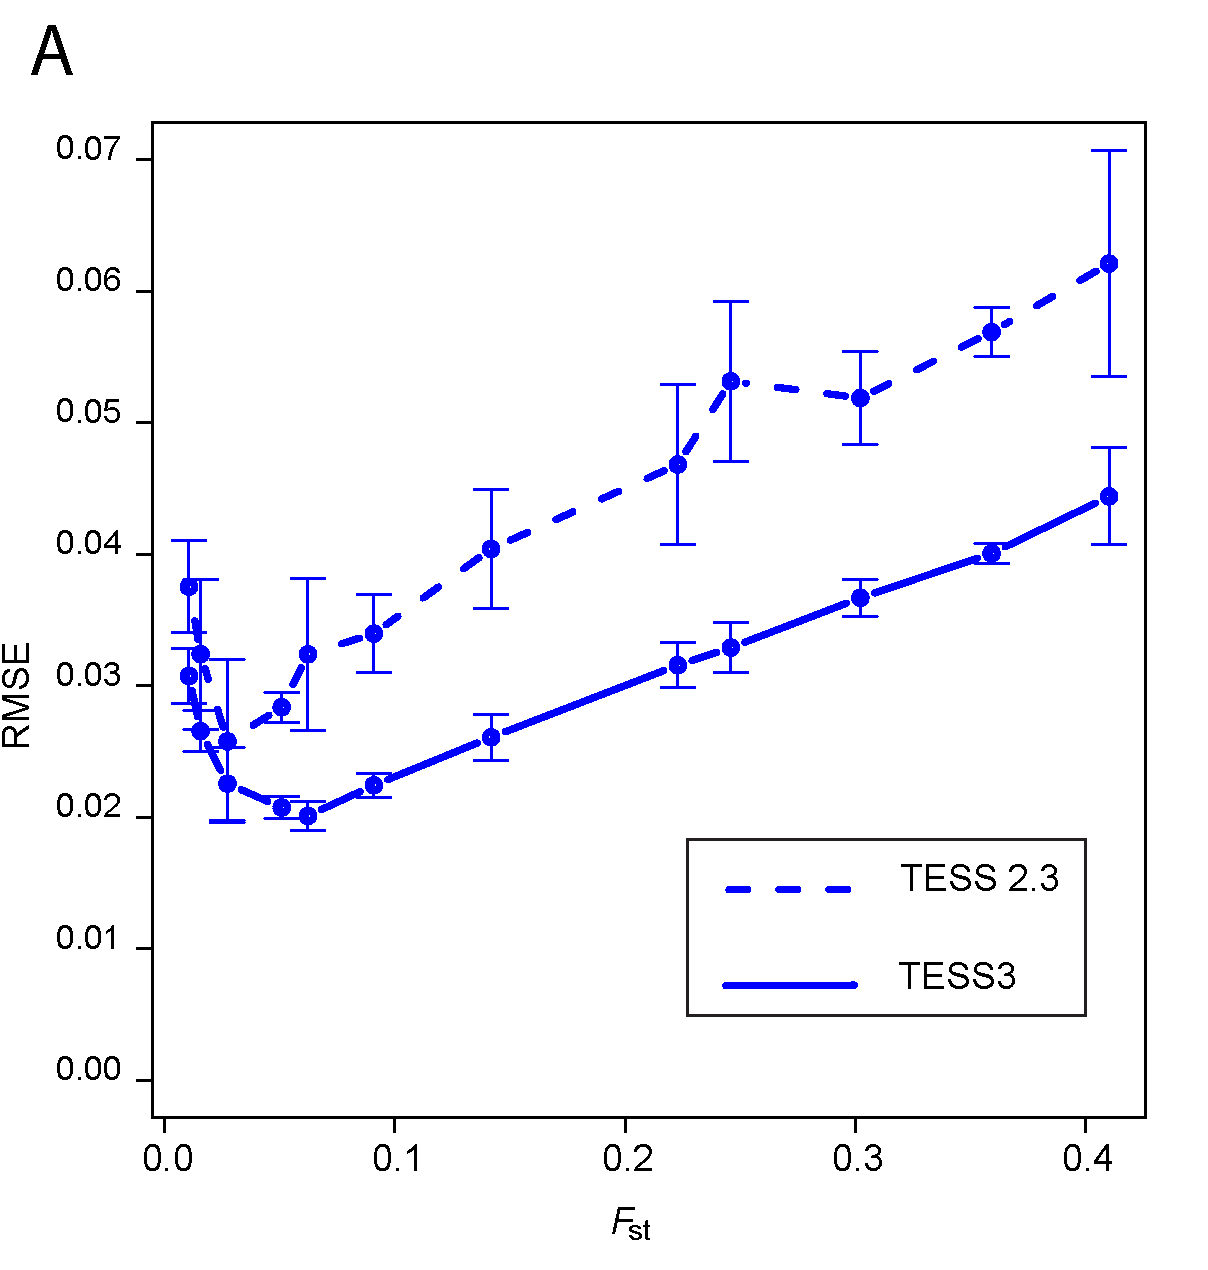
\includegraphics[width=\linewidth]{FinalGraphs/rmseG.pdf}
\end{minipage}
\begin {minipage}{0.49\textwidth}
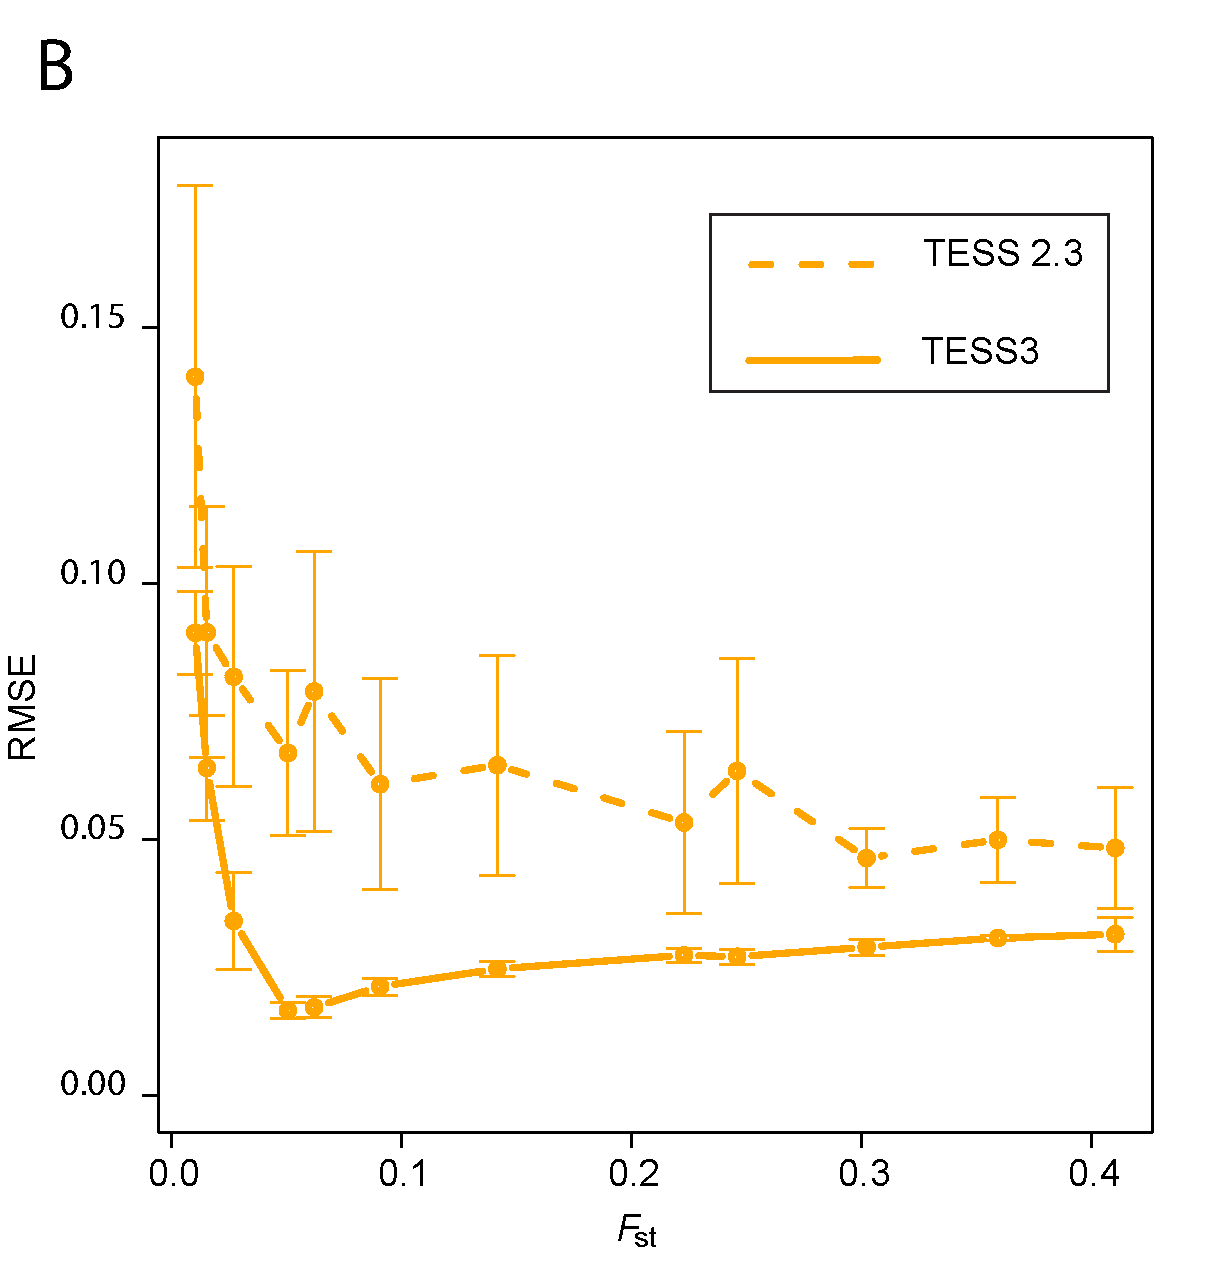
\includegraphics[width=\linewidth]{FinalGraphs/rmseQ.pdf}
\end{minipage}
\caption{Statistical errors of {\tt TESS3} and {\tt TESS 2.3} estimates. Computer simulations of admixed populations using known individual ancestry proportions from two ancestral gene pools. A) RMSEs of $G$ estimates as a function of the level of ancestral population differentiation ($F_{\rm ST}$). B) RMSEs of $Q$ estimates as a function of the level of ancestral population differentiation ($F_{\rm ST}$).}
\end{figure}    

\clearpage
\newpage



\begin{figure}[h!]
  \centering

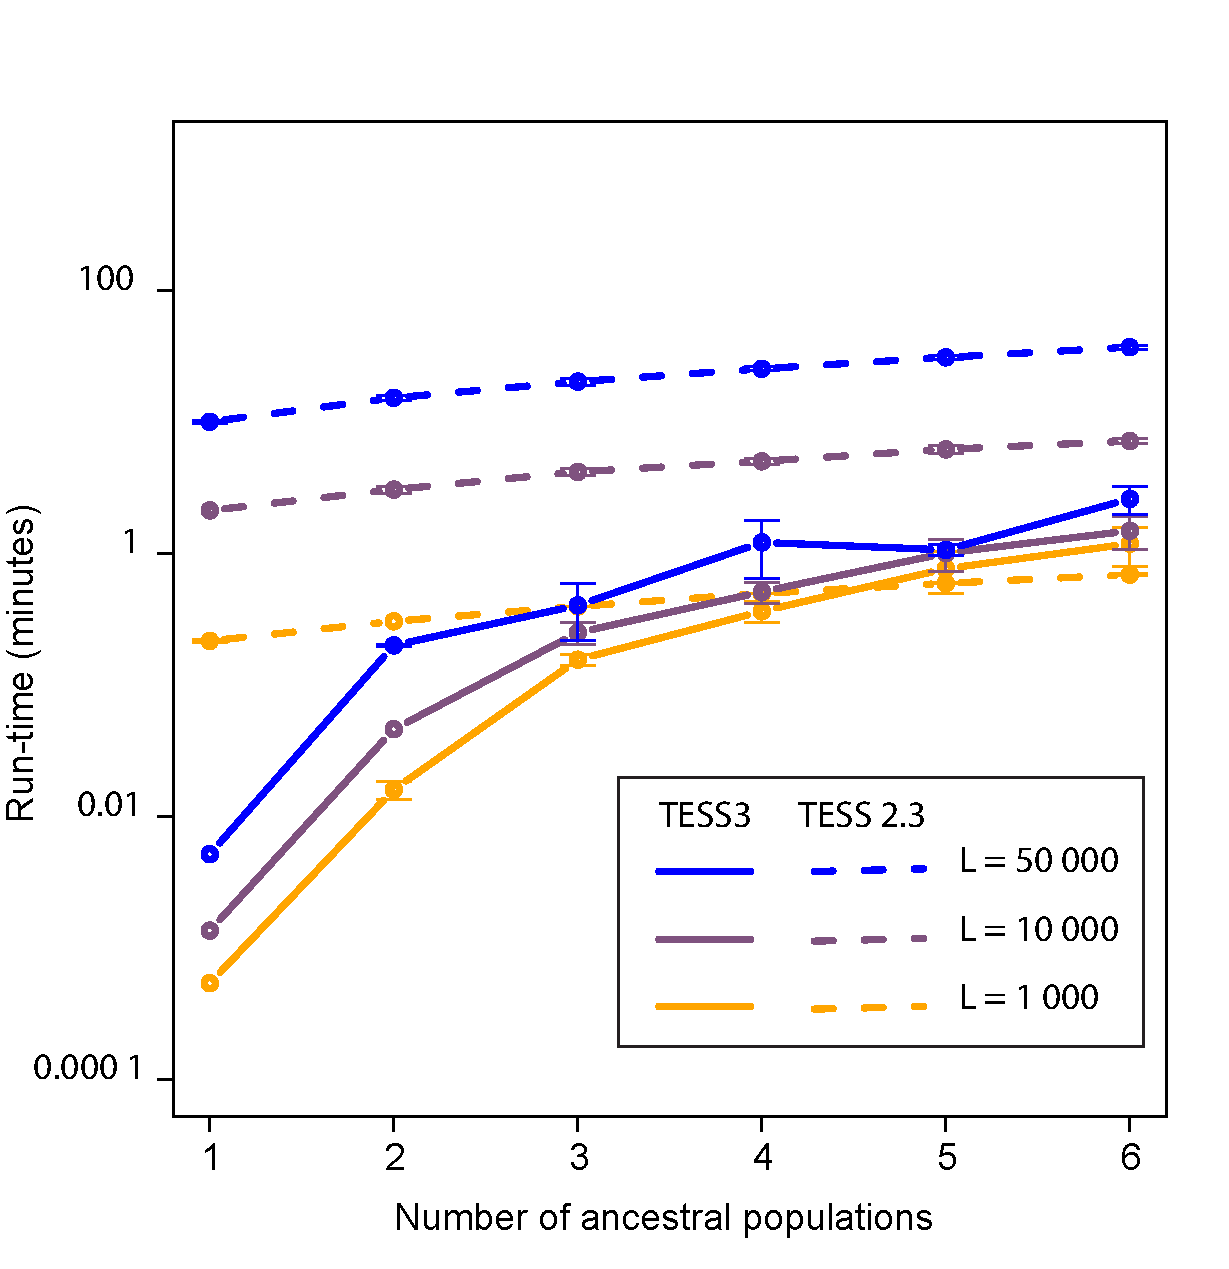
\includegraphics[width=\linewidth]{FinalGraphs/runtimes.pdf}
\caption{ Run-times for {\tt TESS3} and {\tt TESS 2.3} for numbers of ancestral populations ranging between $K = 1$ and $6$. Runtimes were expressed in unit of minutes. }
\end{figure}

\clearpage
\newpage

\begin{table}
\begin{center}
\begin{tabular}{lcc}
 \hline
\textbf{FDR}  & \multicolumn{2}{c}{\textbf{Power}}  \\
 & $m_{\rm s} / m = 0.005$ & $m_{\rm s} / m = 0.05$ \\
\hline
 0.050 & 0.61& 0.16 \\
 0.10 & 0.63 & 0.17\\
 0.15 & 0.64 & 0.19 \\
 0.20 & 0.65 & 0.20 \\
 \hline
\end{tabular}
\end{center}
\caption{Power to reject neutrality for two simulated data sets with distinct values of the ratio ($m_{\rm s} / m$).}
\end{table}


\clearpage	
\newpage


\begin{figure}[h!]\centering
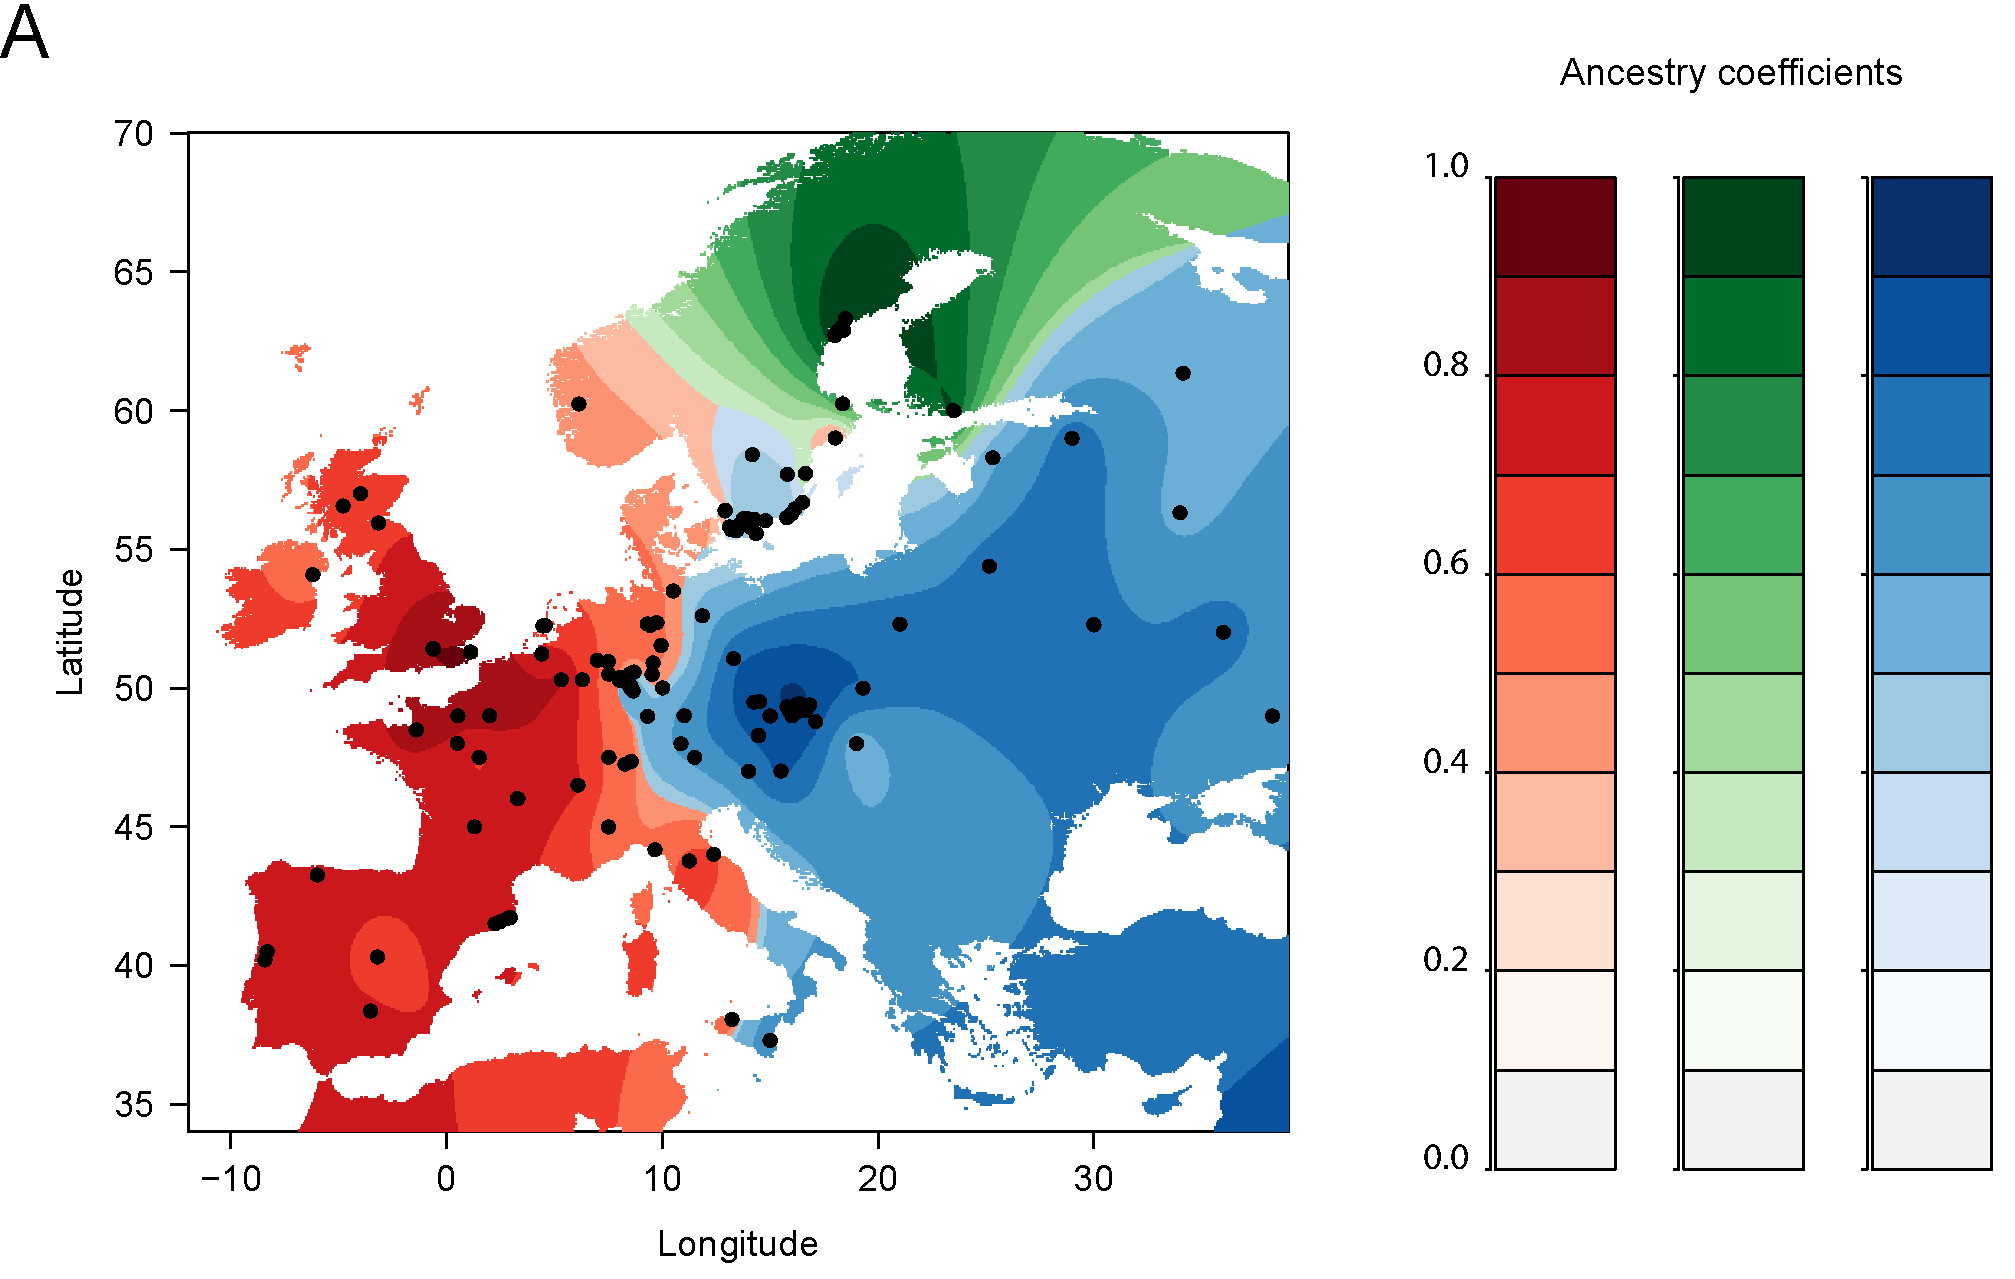
\includegraphics[width=\linewidth]{FinalGraphs/barsClusters.pdf}
\includegraphics[width=\linewidth]{FinalGraphs/manhattanPlot.pdf}
\caption{Results of the {\it Arabidopsis thaliana} data analysis with {\tt TESS3}. A) Geographic maps of ancestry coefficients using $K = 3$ ancestral populations. C) Manhattan plot for the chromosome 5. The horizontal line corresponds to an expected FDR value of $q = 10^{-30}$. }
\end{figure}    

\clearpage
\newpage 

\begin{figure}[h!]\centering
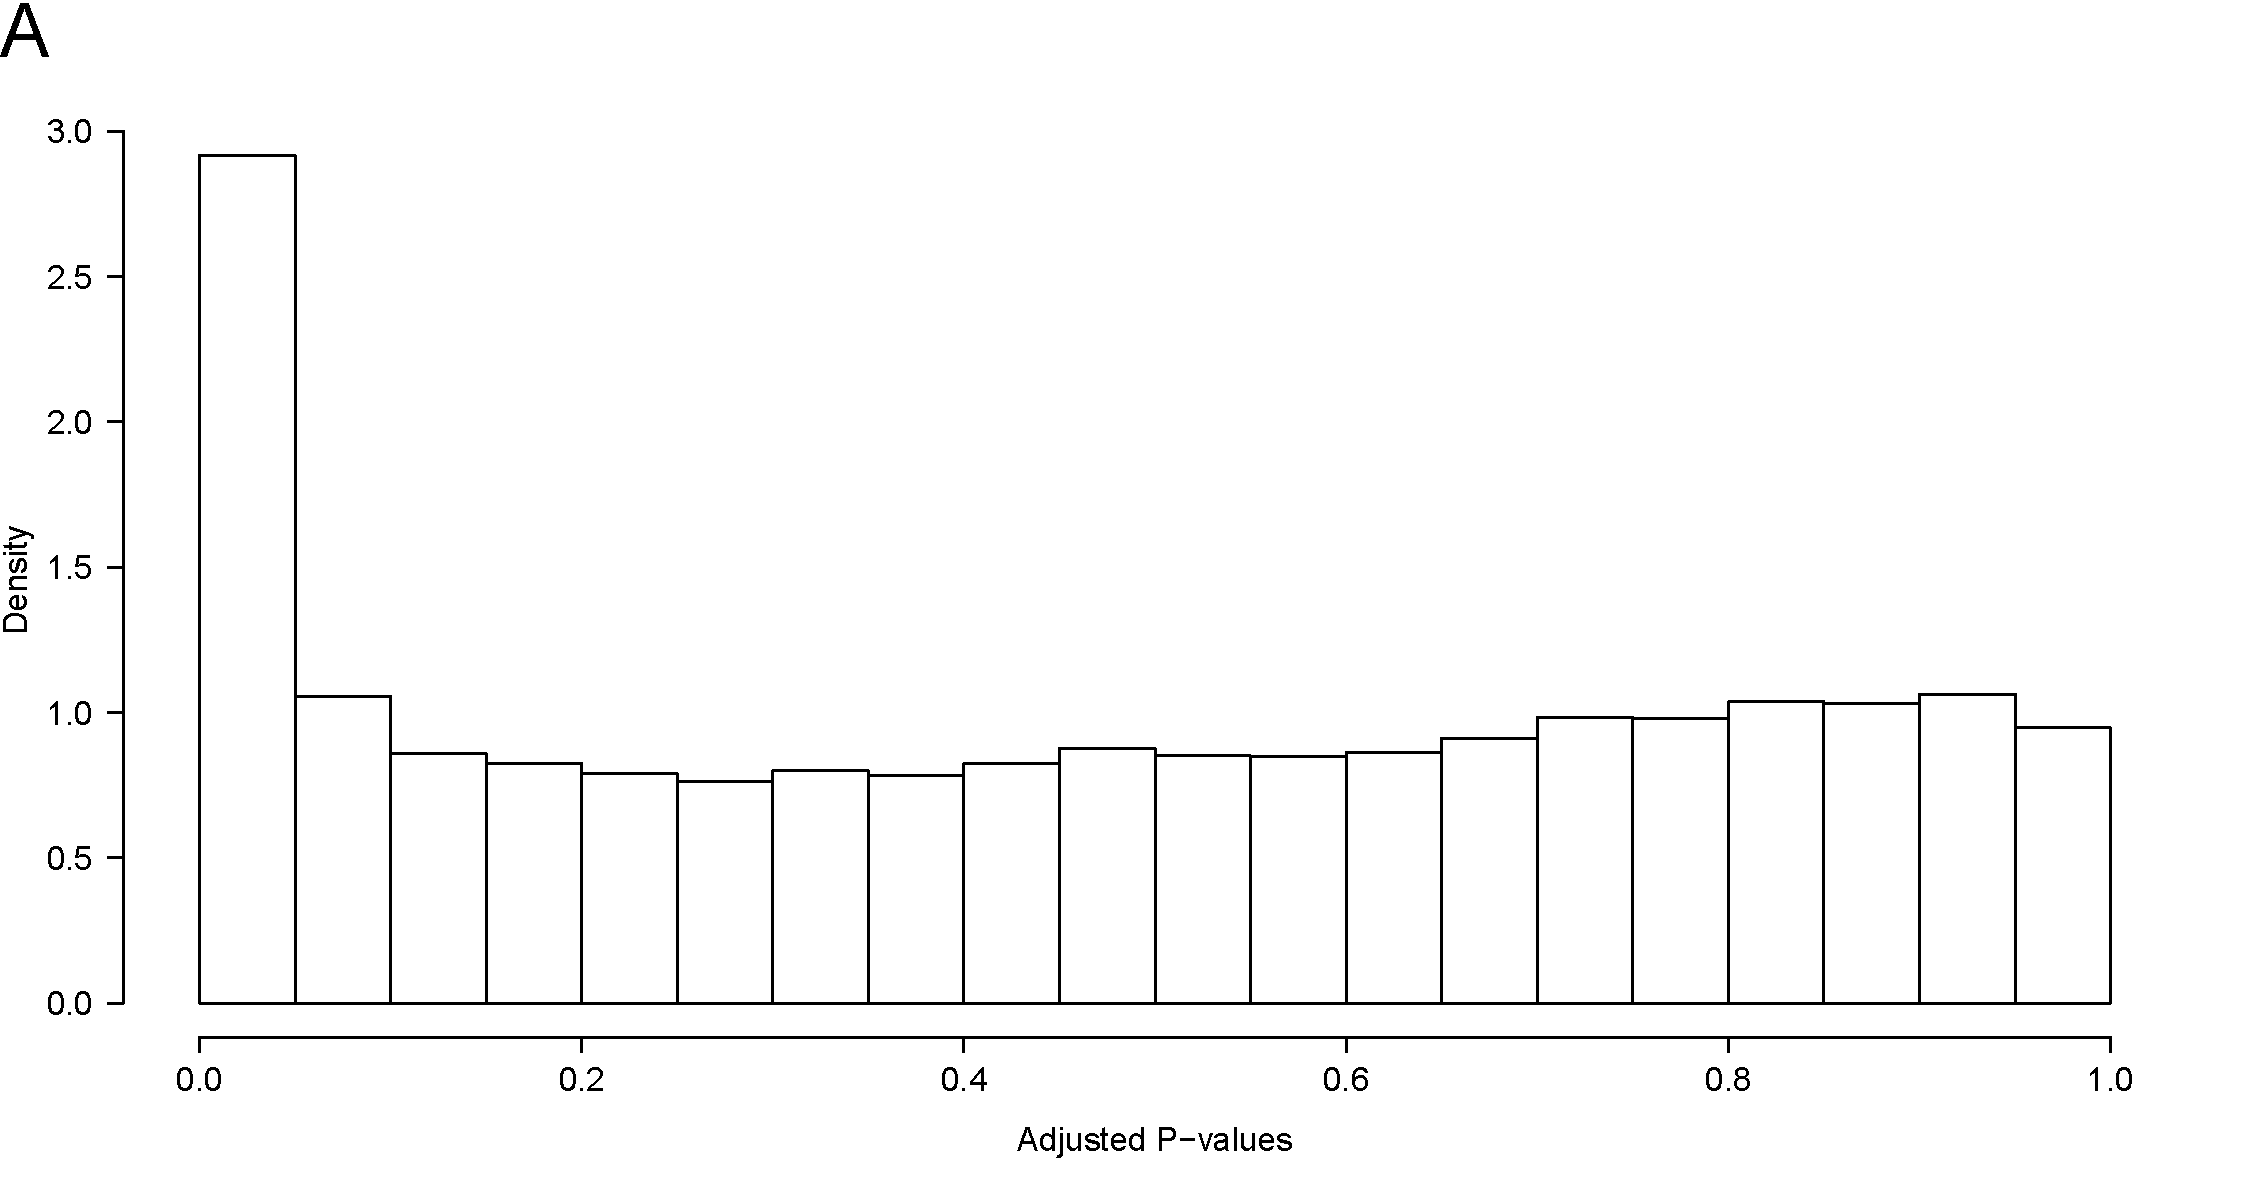
\includegraphics[width=\linewidth]{FinalGraphs/pValueHist.pdf}
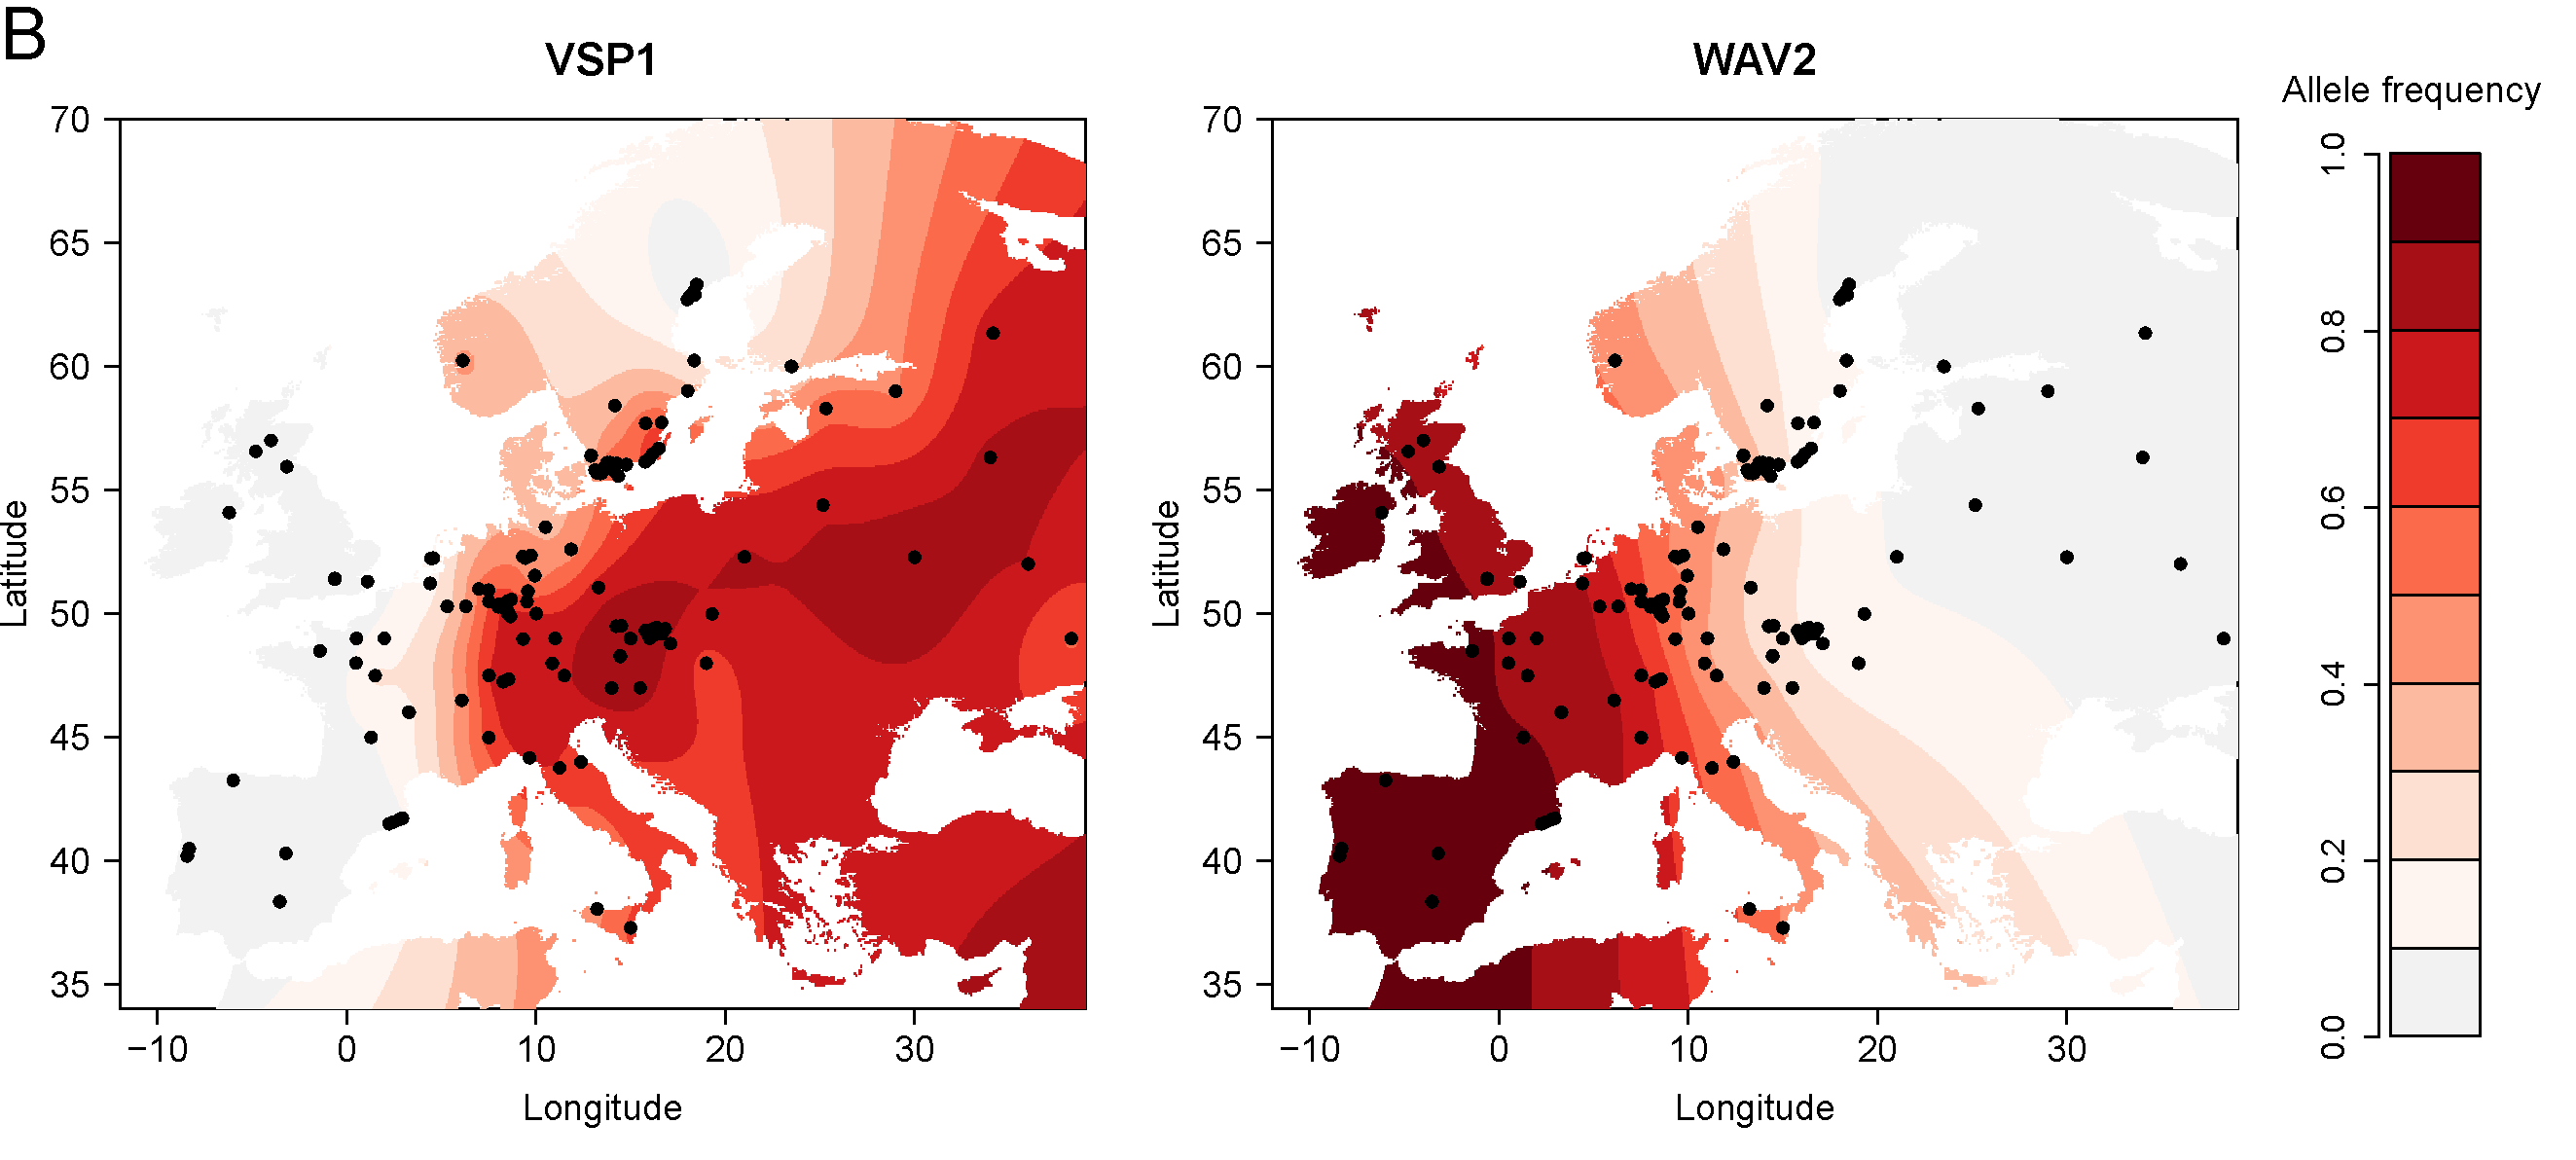
\includegraphics[width=\linewidth]{FinalGraphs/colorBar.pdf}
\caption{ Discoveries from a scan of the {\it A. thaliana} 5th chromosome. A) Histogram of adjusted $p$-values. B) Spatial distribution of two top-hit SNPs located in the {\it VSP1} and {\it WAV2} genes.}
\end{figure}    


\clearpage
\newpage 


\end{document}

    
